% !TEX program = xelatex
% DriveCompose manuscript for CVPR 2027; inherited CVPR style files.
\documentclass[10pt,twocolumn,letterpaper]{article}
\usepackage[review]{cvpr}
%% This file contains a number of tweaks that are typically applied to the main document.
%% They are not enabled by default, but can be enabled by uncommenting the relevant lines.


%% Standard CVPR float handling is used for the teaser and experiment figures.
\usepackage{placeins} %< keep references after all experiment floats

%%
%% caption and (global) spacing overrides
%%
\usepackage{caption} %< for "\captionof" commands (teaser)
% \setlength{\abovecaptionskip}{.5em} % space above caption
% \setlength{\belowcaptionskip}{1em} % space below caption

%%
%% Inline annotations; for predefined colors, refer to "dvipsnames" in the xcolor package:
%% https://tinyurl.com/overleaf-colors
%%
\newcommand{\red}[1]{{\color{red}#1}}
\newcommand{\todo}[1]{{\color{red}#1}}
\newcommand{\TODO}[1]{\textbf{\color{red}[TODO: #1]}}
%%
%% Disable for camera ready / submission by uncommenting these lines:
%%
% \renewcommand{\TODO}[1]{}
% \renewcommand{\todo}[1]{#1}

%%
%% Work harder in optimizing text layout. Typically shrinks text by 1/6 of page, enable
%% it at the very end of the writing process, when you are just above the page limit.
%%
% \usepackage{microtype}

%%
%% Fine-tune paragraph spacing.
%%
% \renewcommand{\paragraph}[1]{\vspace{.5em}\noindent\textbf{#1.}}

%%
%% Globally adjusts space between figure and caption.
%%
% \setlength{\abovecaptionskip}{.5em}

%%
%% Allows "the use of \paper to refer to the project name"
%% with automatic management of space at the end of the word.
%%
% \usepackage{xspace}
% \newcommand{\paper}{ProjectName\xspace}

%%
%% Commonly used math definitions.
%%
% \DeclareMathOperator*{\argmin}{arg\,min}
% \DeclareMathOperator*{\argmax}{arg\,max}

%%
%% Tighten underline.
%%
% \usepackage{soul}
% \setuldepth{foobar}

%%
%% Reconfigure paragraph (tweaks spacing)
%%






% Portable Times-compatible Unicode fonts; CVPR geometry is unchanged.
\usepackage{iftex}
\ifXeTeX
  \usepackage{fontspec}
  \setmainfont{texgyretermes-regular.otf}[
    BoldFont=texgyretermes-bold.otf,ItalicFont=texgyretermes-italic.otf,
    BoldItalicFont=texgyretermes-bolditalic.otf]
  \setsansfont{texgyreheros-regular.otf}[
    BoldFont=texgyreheros-bold.otf,ItalicFont=texgyreheros-italic.otf,
    BoldItalicFont=texgyreheros-bolditalic.otf]
  \setmonofont{texgyrecursor-regular.otf}[
    BoldFont=texgyrecursor-bold.otf,ItalicFont=texgyrecursor-italic.otf,
    BoldItalicFont=texgyrecursor-bolditalic.otf]
\fi

\usepackage{tikz}
\usepackage{needspace}
\usetikzlibrary{arrows.meta,patterns}
\definecolor{cvprblue}{rgb}{0.21,0.49,0.74}
\usepackage[pagebackref,breaklinks,colorlinks,allcolors=cvprblue]{hyperref}
\usepackage{url}
\def\paperID{*****}
\def\confName{CVPR}
\def\confYear{2027}
\title{DriveCompose: Observation-Anchored Joint Completion of Composable Gaussian Driving Worlds}
\author{Anonymous CVPR Submission}
\begin{document}
\maketitle
\begin{abstract}
Reusing a driving scene under new camera and actor states exposes surfaces that were never recorded. Reconstructing such a scene requires recovering the observed content, completing missing geometry and appearance, and retaining a stable identity for each movable component. We present DriveCompose, a framework for generative reconstruction of compositional driving scenes from calibrated image sequences. It jointly completes a world-space background and canonical vehicle and human assets, so generated surfaces inherit the coordinate frames and motion bindings used for later scene editing. A conditional flow model combines local attention with cross-component memory, while observed codes, known free space, and input-view checks constrain the completed Gaussian scene. On Waymo, DriveCompose reduces FID from 83.72 to 37.43 relative to STORM for $\pm2\,\mathrm{m}$ camera shifts. Cross-component memory lowers unseen-surface RGB error by 20.5\% relative to isolated per-component memories with eight input timestamps. The resulting scene can be rendered under different camera and actor states without resampling its completed geometry or appearance.
\end{abstract}

\begin{figure*}[t]
  \centering
  % Native vector overview; physical canvas 495 x 225 pt at CVPR text width.
% All scene marks are schematic. No experiment results are drawn here.
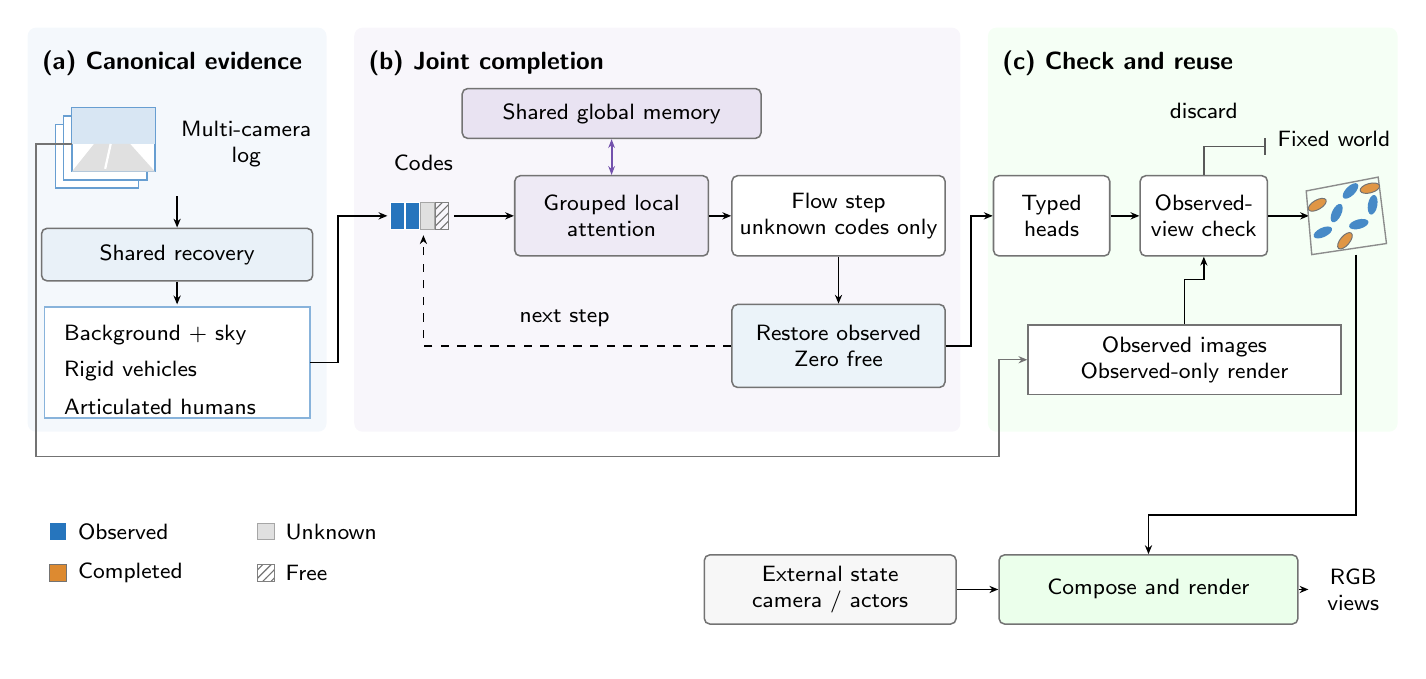
\begin{tikzpicture}[x=1pt,y=1pt,
  every node/.style={font=\sffamily\fontsize{8.3}{9.5}\selectfont,inner sep=2pt,align=center},
  op/.style={draw=black!55,rounded corners=2pt,fill=white,line width=.55pt},
  route/.style={-{Stealth[length=3.2pt,width=2.6pt]},line width=.65pt},
  paneltitle/.style={anchor=west,font=\sffamily\bfseries\fontsize{9.5}{11}\selectfont,inner sep=0pt}]
\path[use as bounding box] (0,0) rectangle (495,225);
\definecolor{dcobs}{HTML}{2675BD}
\definecolor{dcnew}{HTML}{DD8A30}
\definecolor{dcmem}{HTML}{7351AD}
\fill[dcobs!5,rounded corners=3pt] (0,79) rectangle (108,225);
\fill[dcmem!5,rounded corners=3pt] (118,79) rectangle (337,225);
\fill[green!4,rounded corners=3pt] (347,79) rectangle (495,225);
\node[paneltitle] at (5,212) {(a) Canonical evidence};
\node[paneltitle] at (123,212) {(b) Joint completion};
\node[paneltitle] at (352,212) {(c) Check and reuse};

% Camera observations: stacked image planes, kept distinct from query tensors.
\foreach \dx/\dy in {0/0,3/3,6/6}{
  \draw[fill=white,draw=dcobs!70,line width=.6pt] (10+\dx,167+\dy) rectangle (40+\dx,190+\dy);
}
\fill[dcobs!18] (16,183) rectangle (46,196);
\fill[black!12] (16,173) -- (24,183) -- (37,183) -- (46,173) -- cycle;
\draw[white,line width=.8pt] (28,174) -- (30,183);
\node[text width=54pt] at (79,183) {Multi-camera\\log};
\node[op,fill=dcobs!10,minimum width=98pt,minimum height=19pt] (recovery) at (54,143) {Shared recovery};
\draw[route] (54,164) -- (recovery.north);
\draw[route] (recovery.south) -- (54,125);
\draw[draw=dcobs!55,fill=white,line width=.55pt] (6,84) rectangle (102,124);
\node[anchor=west,inner sep=0pt] at (13,114) {Background + sky};
\node[anchor=west,inner sep=0pt] at (13,101) {Rigid vehicles};
\node[anchor=west,inner sep=0pt] at (13,88) {Articulated humans};
\draw[route] (102,104) -- (112,104) -- (112,157) -- (130,157);

% Partial-code strip; pattern distinguishes free from unknown in grayscale.
\foreach \i in {0,1}{\filldraw[fill=dcobs,draw=white,line width=.3pt] (131+5.4*\i,152) rectangle +(5,10);}
\filldraw[fill=black!12,draw=black!35,line width=.3pt] (141.8,152) rectangle +(5,10);
\filldraw[pattern=north east lines,pattern color=black!55,draw=black!50,line width=.3pt] (147.2,152) rectangle +(5,10);
\node at (143,176) {Codes};
\node[op,fill=dcmem!12,minimum width=70pt,minimum height=29pt] (local) at (211,157) {Grouped local\\attention};
\draw[route] (154,157) -- (local.west);
\node[op,fill=dcmem!16,minimum width=108pt,minimum height=18pt] (memory) at (211,194) {Shared global memory};
\draw[{Stealth[length=3.2pt]}-{Stealth[length=3.2pt]},line width=.7pt,draw=dcmem] (local.north) -- (memory.south);
\node[op,minimum width=77pt,minimum height=29pt] (euler) at (293,157) {Flow step\\unknown codes only};
\draw[route] (local.east) -- (euler.west);
\node[op,fill=dcobs!9,minimum width=77pt,minimum height=30pt] (restore) at (293,110) {Restore observed\\Zero free};
\draw[route] (euler.south) -- (restore.north);
\draw[route,dashed] (restore.west) -- (143,110) -- (143,150);
\node at (194,120) {next step};

% Decode only after integration and projection. Rejected candidates never enter W.
\node[op,minimum width=42pt,minimum height=29pt] (heads) at (370,157) {Typed\\heads};
\draw[route] (restore.east) -- (341,110) -- (341,157) -- (heads.west);
\node[op,minimum width=46pt,minimum height=29pt] (check) at (425,157) {Observed-\\view check};
\draw[route] (heads.east) -- (check.west);
\node[draw=black!55,fill=white,line width=.55pt,text width=109pt,minimum height=25pt] (reference) at (418,105) {Observed images\\Observed-only render};
\draw[route] (reference.north) -- (418,134) -- (425,134) -- (check.south);
\draw[route,draw=black!55,line width=.5pt] (16,183) -- (3,183) -- (3,70) -- (351,70) -- (351,105) -- (reference.west);
\draw[line width=.6pt,draw=black!65] (check.north) -- (425,182) -- (447,182);
\draw[line width=.8pt,draw=black!65] (447,179) -- (447,185);
\node at (425,195) {discard};
\draw[route] (check.east) -- (463,157);
\node at (472,185) {Fixed world};
\draw[black!45,line width=.5pt] (464,143) -- (491,147) -- (488,171) -- (462,166) -- cycle;
\foreach \x/\y/\a in {468/151/25,473/158/65,481/154/15,478/166/45,486/161/80}{
  \fill[dcobs!85,rotate around={\a:(\x,\y)}] (\x,\y) ellipse (3.6pt and 1.7pt);
}
\foreach \x/\y/\a in {466/161/30,476/148/50,485/167/15}{
  \filldraw[fill=dcnew!90,draw=black!55,line width=.35pt,rotate around={\a:(\x,\y)}] (\x,\y) ellipse (3.6pt and 1.7pt);
}

% Runtime consumes accepted fixed content and externally supplied states.
\node[op,fill=black!3,minimum width=91pt,minimum height=25pt] (state) at (290,22) {External state\\camera / actors};
\node[op,fill=green!8,minimum width=108pt,minimum height=25pt] (renderer) at (405,22) {Compose and render};
\node[text width=28pt] (views) at (479,22) {RGB\\views};
\draw[route] (state.east) -- (renderer.west);
\draw[route] (renderer.east) -- (views.west);
\draw[route] (480,143) -- (480,49) -- (405,49) -- (renderer.north);

% Semantic legend at final publication size.
\fill[dcobs] (8,40) rectangle +(6,6); \node[anchor=west,inner sep=0pt] at (18,43) {Observed};
\filldraw[fill=black!12,draw=black!35,line width=.3pt] (83,40) rectangle +(6,6); \node[anchor=west,inner sep=0pt] at (93,43) {Unknown};
\filldraw[fill=dcnew,draw=black!55,line width=.35pt] (8,25) rectangle +(6,6); \node[anchor=west,inner sep=0pt] at (18,28) {Completed};
\filldraw[pattern=north east lines,pattern color=black!55,draw=black!50,line width=.3pt] (83,25) rectangle +(6,6);
\node[anchor=west,inner sep=0pt] at (93,28) {Free};
\end{tikzpicture}

  \caption{\textbf{DriveCompose construction and reuse.} (a) A shared front end recovers evidence on world-space and canonical supports. (b) Local query groups exchange context through global memory; each flow step restores observed codes and clears free space. (c) Typed heads decode the completed codes. An observed-view check compares the candidate with the images and an observed-only decode; rejected candidates do not enter the fixed world. External policy and dynamics supply the states used for subsequent composition and RGB rendering. All scene marks are schematic.}
  \label{fig:teaser}
\end{figure*}
\def\CVPRMAIN{}
\section{Introduction}
\label{sec:introduction}

Driving simulation and scene editing require 3D scenes that support changes in camera viewpoint, vehicle motion, and human pose~\cite{yang2023unisim,zhou2024hugsim}. However, driving images reveal only the surfaces visible from the recorded viewpoints and actor configurations~\cite{sun2020waymo,caesar2020nuscenes}. Moving a camera, turning a vehicle, or changing a pedestrian's pose exposes previously unobserved regions. Reconstructing scenes for these operations therefore requires completing the missing geometry and appearance while ensuring that completed vehicle and human surfaces move with their respective actors.

Recent feed-forward methods fuse multiple images to directly predict driving-scene geometry and Gaussian representations~\cite{yang2025storm,chen2025dggt,yu2026streetforward,chi2026pointforward}. Motion estimation and visibility modeling further help align dynamic objects and integrate observations over time. Multi-frame aggregation increases coverage of surfaces visible in the input sequence. When a new viewpoint or actor motion reveals surfaces unseen throughout the sequence, reconstruction must infer their geometry and appearance.

Generative reconstruction uses asset priors, Gaussian completion, or generated views to infer unobserved content~\cite{yang2025genassets,liao2025complete,streetcrafter,zhu2025worldsplat}. Meanwhile, compositional reconstruction represents the background and moving actors separately to support vehicle motion and human pose control~\cite{yan2024street,chen2025omnire,zhou2024hugsim}. Applying generative completion to such scenes requires generated surfaces to move with their actors. When an actor is only partially observed, information from the background and other actors can provide additional context for inferring its missing content.

To this end, we introduce DriveCompose, a framework that generatively reconstructs compositional driving scenes from image sequences while supporting independent actor control. We represent the background in world coordinates, vehicle surfaces in each vehicle's own coordinate frame, and human surfaces in a reference pose with skeletal bindings~\cite{yan2024street,chen2025omnire}. Completion operates directly on these representations, allowing generated vehicle and human surfaces to follow their actors' motion and pose changes (Sec.~\ref{sec:representation}). The model jointly completes missing background and actor content using shared scene context.

As illustrated in Fig.~\ref{fig:overview}, DriveCompose first recovers scene geometry and actor motion from the image sequence and aligns multi-frame image features with the background, vehicle, and human representations. The completion model captures local structure within each component, while cross-component memory gathers information from the background and actors and distributes the shared context back to each component. Missing regions of a vehicle or human can therefore be completed using information from the surrounding scene. The model learns to generate missing latent codes through conditional flow matching~\cite{lipman2022flowmatching}, and component-specific decoders convert the completed representations into a Gaussian scene~\cite{kerbl2023gaussians}.

To maintain consistency with input observations, we preserve the geometry and appearance of reliably observed surfaces during completion. We then render the completed scene at the recorded camera viewpoints and actor states and compare it with the input images to check for inconsistencies introduced by completion. Scenes that pass this check can reuse the same completed content for rendering under different camera viewpoints and actor states (Sec.~\ref{sec:composition}).

On Waymo, DriveCompose improves dynamic scene reconstruction and off-trajectory view synthesis over the evaluated baselines (Sec.~\ref{sec:experiments}). Component ablations further show that cross-component information sharing reduces mean absolute RGB error on unseen surfaces, with larger absolute error reductions under sparser observations (Sec.~\ref{sec:ablations}).

\Needspace{6\baselineskip}
Our contributions are:
\begin{itemize}
\item We introduce DriveCompose, a generative reconstruction framework for closed-loop driving simulation. It recovers and completes backgrounds, vehicles, and humans from image sequences to construct compositional Gaussian scene assets. The resulting scene reuses the same completed assets for composition and rendering as camera poses, vehicle poses, and human poses change.
\item We develop a cross-component latent completion model based on conditional flow matching. Local attention models spatial relationships within each component, while cross-component memory aggregates background and actor features to provide scene context for generating each component's missing content.
\item We evaluate the framework through dynamic reconstruction and off-trajectory view synthesis, and use component ablations to quantify the reduction in mean absolute RGB error on unseen surfaces from cross-component information sharing.
\end{itemize}

Section~\ref{sec:related} reviews related work, Section~\ref{sec:method} presents the method, and Section~\ref{sec:experiments} reports experiments. Sections~\ref{sec:discussion} and~\ref{sec:conclusion} discuss limitations and conclude.

\section{Related work}
\label{sec:related}

\paragraph{Learned driving-scene reconstruction.}
Feed-forward models replace repeated scene fitting with learned inference from image observations. STORM predicts Gaussians and scene flow for dynamic outdoor reconstruction~\cite{yang2025storm}. DGGT adds pose-free reconstruction, temporal visibility, and motion-guided interpolation~\cite{chen2025dggt}. StreetForward, PointForward, and Instant NuRec explore temporal processing, point-aligned representations, and feed-forward reconstruction for simulation~\cite{yu2026streetforward,chi2026pointforward,huang2026instantnurec}. We build on the role of image-based recovery as a source of geometry and motion evidence. Our output variables are background and canonical asset codes, which support conditional completion before the scene is rendered under new states.

\paragraph{Compositional scenes and control.}
Street Gaussians models tracked vehicles separately from static background~\cite{yan2024street}. OmniRe extends this organization to multiple actor types with category-appropriate motion models~\cite{chen2025omnire}. HUGSIM provides control-driven state updates and interactive simulation using reconstructed content~\cite{zhou2024hugsim}. These methods separate persistent appearance and geometry from motion. We retain this separation within the generative representation, so completed surfaces inherit an asset identity and its rigid or articulated transform.

\paragraph{Generative reconstruction and completion.}
StreetCrafter uses three-dimensional conditions to generate views that guide reconstruction, and HorizonForge combines editable scene content with video diffusion~\cite{streetcrafter,wang2026horizonforge}. WorldSplat generates pixel-aligned Gaussians from a latent model and refines their rendered videos~\cite{zhu2025worldsplat}. GenAssets learns priors for driving assets, CompleteSplat completes Gaussian scenes from image evidence, and JRM uses latent flow matching to combine unaligned observations of shared objects~\cite{yang2025genassets,liao2025complete,wu2026jrm}. LatentWorld organizes semantic occupancy generation around scene entities~\cite{park2026latentworld}. DriveCompose conditions on a recovered driving log and completes RGB-renderable background and canonical assets in one query layout. Generation acts on their unknown latent content; observed evidence constrains both sampling and the assembled render.

\section{Method}\label{sec:method}

DriveCompose converts multi-view image sequences into a compositional Gaussian scene through visual encoding, canonical feature aggregation, latent encoding, joint latent completion, type-specific Gaussian decoding, and scene composition (Fig.~\ref{fig:overview}). Canonical aggregation aligns observations of each component across time; joint completion uses the surrounding scene to infer its missing geometry and appearance.

\subsection{Problem formulation and compositional representation}
\label{sec:representation}

The input is a synchronized image log $\mathbf I_{t,v}$ with timestamps, camera intrinsics, and camera-to-rig calibration. Rig poses are provided or estimated relative to the first frame. Coordinate conventions and image preprocessing are detailed in Appendix D of the supplementary material.

The output is a compositional Gaussian scene

\begin{equation}
\mathcal W=\bigl(\mathcal G_b,C_{\rm sky},V_{\rm sky},
\{\mathcal A_a\},\mathcal B,\xi\bigr),
\label{eq:world}
\end{equation}

where $\mathcal G_b$ is the world-space background, $C_{\rm sky}$ a sky cubemap, $V_{\rm sky}$ its supported directions, $\mathcal A_a$ the canonical asset for identity $a$, $\mathcal B$ the finite spatial support, and $\xi$ the sampling seed. The components are rendered by Gaussian splatting~\cite{kerbl2023gaussians}. Vehicles are represented as rigid assets with fixed local geometry and dimensions. Humans additionally retain a rest skeleton and skinning weights. Scene state controls the placement and articulation of these fixed components.

We model missing content through conditional generation. Let $\mathcal Q$ be the recovered query layout and $C$ its observed evidence. The completion model samples unknown codes $\mathbf z_u$, while the codec $D_\psi$ decodes the assembled codes into scene content:

\begin{equation}
\mathbf z_u\sim p_\theta(\mathbf z_u\mid C,\mathcal Q),
\qquad
\mathcal W=D_\psi(\mathbf z^{\rm obs},\mathbf z_u;\mathcal Q).
\label{eq:generative-reconstruction}
\end{equation}

The query layout assigns each latent code to a spatial location and scene component. Completion fills the unknown codes within this layout, and decoding preserves their component identities and motion bindings.

\subsection{Visual encoding}
\label{sec:visual-encoding}

The Driving Log Encoder extracts patch features from each image and exchanges pooled context across cameras and timestamps~\cite{dosovitskiy2021vit,vaswani2017attention}. Geometry heads predict camera-axis depth, normals, confidence, semantics, and instance assignments. These predictions connect the image features to 3D surfaces and their owning components. Trajectory-level identity slots separate persistent identity, dimensions, and human shape from frame-dependent root poses and joint rotations. Architectural details and state parameterization are given in Appendix D of the supplementary material.

\subsection{Canonical feature aggregation}
\label{sec:queries}

\paragraph{Spatial supports.}

A query stores canonical position $\mathbf q_i$, cell scale $\boldsymbol\delta_i$, type $k_i$, local attention group $g_i$, and reference-world coordinate $\mathbf q_i^w$. Reliable depth samples provide surface anchors. Background anchors are combined with a finite world grid; rigid anchors are aligned by inverse SE(3) transforms and combined with a grid in the local bounding volume. Human queries lie on the canonical template surface. Sky queries are unit directions grouped by cubemap face. These supports provide explicit locations for both observed and missing content.

The layout remains fixed during completion. We obtain $\mathbf q_i^w$ by placing the query in the first input configuration, including skinning for humans. Canonical coordinates identify the content within its component; reference-world coordinates let the generator relate that component to its surroundings.

\paragraph{Motion-aware evidence aggregation.}

For each observation, we place the canonical query at the corresponding actor state:

\begin{equation}
\mathbf p_i(t)=
\begin{cases}
\mathbf q_i,& k_i=\mathrm{background},\\
\operatorname{xyz}(\mathbf T^w_a(t)\bar{\mathbf q}_i),& k_i=\mathrm{rigid},\\
\operatorname{xyz}(\mathbf T^w_h(t)\mathbf A_i(t)\bar{\mathbf q}_i),& k_i=\mathrm{human}.
\end{cases}
\label{eq:query-placement}
\end{equation}

Here $\bar{\mathbf q}_i$ is homogeneous, $\operatorname{xyz}$ extracts Euclidean coordinates, and $\mathbf A_i(t)$ is the weighted skinning transform. Projection gives query depth $z_{i,t,v}$ and samples image features $\boldsymbol\phi_{i,t,v}$, depth $d_{i,t,v}$, and confidence $c_{i,t,v}$. We weight observations by confidence and normalized depth residual $r=(d-z)/(\eta_{\rm abs}+\eta_{\rm rel}d)$. The indicator $a_{i,t,v}$ selects visible, depth-consistent observations of the same instance (Appendix D):

\begin{align}
w_{i,t,v}&=a_{i,t,v}c_{i,t,v}\exp(-r_{i,t,v}^2/2),\\
\mathbf h_i&=\frac{\sum_{t,v}w_{i,t,v}[\boldsymbol\phi_{i,t,v};r_{i,t,v}]}
{\max(\varepsilon,\sum_{t,v}w_{i,t,v})}.
\label{eq:aggregation}
\end{align}

The masks $m_i$, $f_i$, and $u_i$ distinguish observed surfaces, known free space, and unknown content, with $m_i+f_i+u_i=1$. Confidence is the maximum over valid observations; free space is inferred from reliable depth rays. Sky features are aggregated by viewing direction using camera rotation and sky semantics. Appendix D gives the visibility and free-space criteria.

\subsection{Latent representation encoding}
\label{sec:codec}

Type-specific encoders compress the aggregated feature and its spatial support, $[\mathbf h_i;\mathbf q_i;\boldsymbol\delta_i]$, into a latent code $\mathbf z_i\in\mathbb R^D$. The shared latent dimension lets the completion model exchange information across background, rigid, and human representations. Each query keeps its type, ownership, and coordinate frame even though all codes have the same dimension. Visibility masks and confidence are supplied separately to the completion model. Partial and complete observations therefore use the same intrinsic encoding map. Before conditioning, unobserved codes are set to zero; the observed subset is denoted $\mathbf z^{\rm obs}$.

\subsection{Joint latent-space completion}
\label{sec:completion}

\begin{figure*}[t]
  \centering
  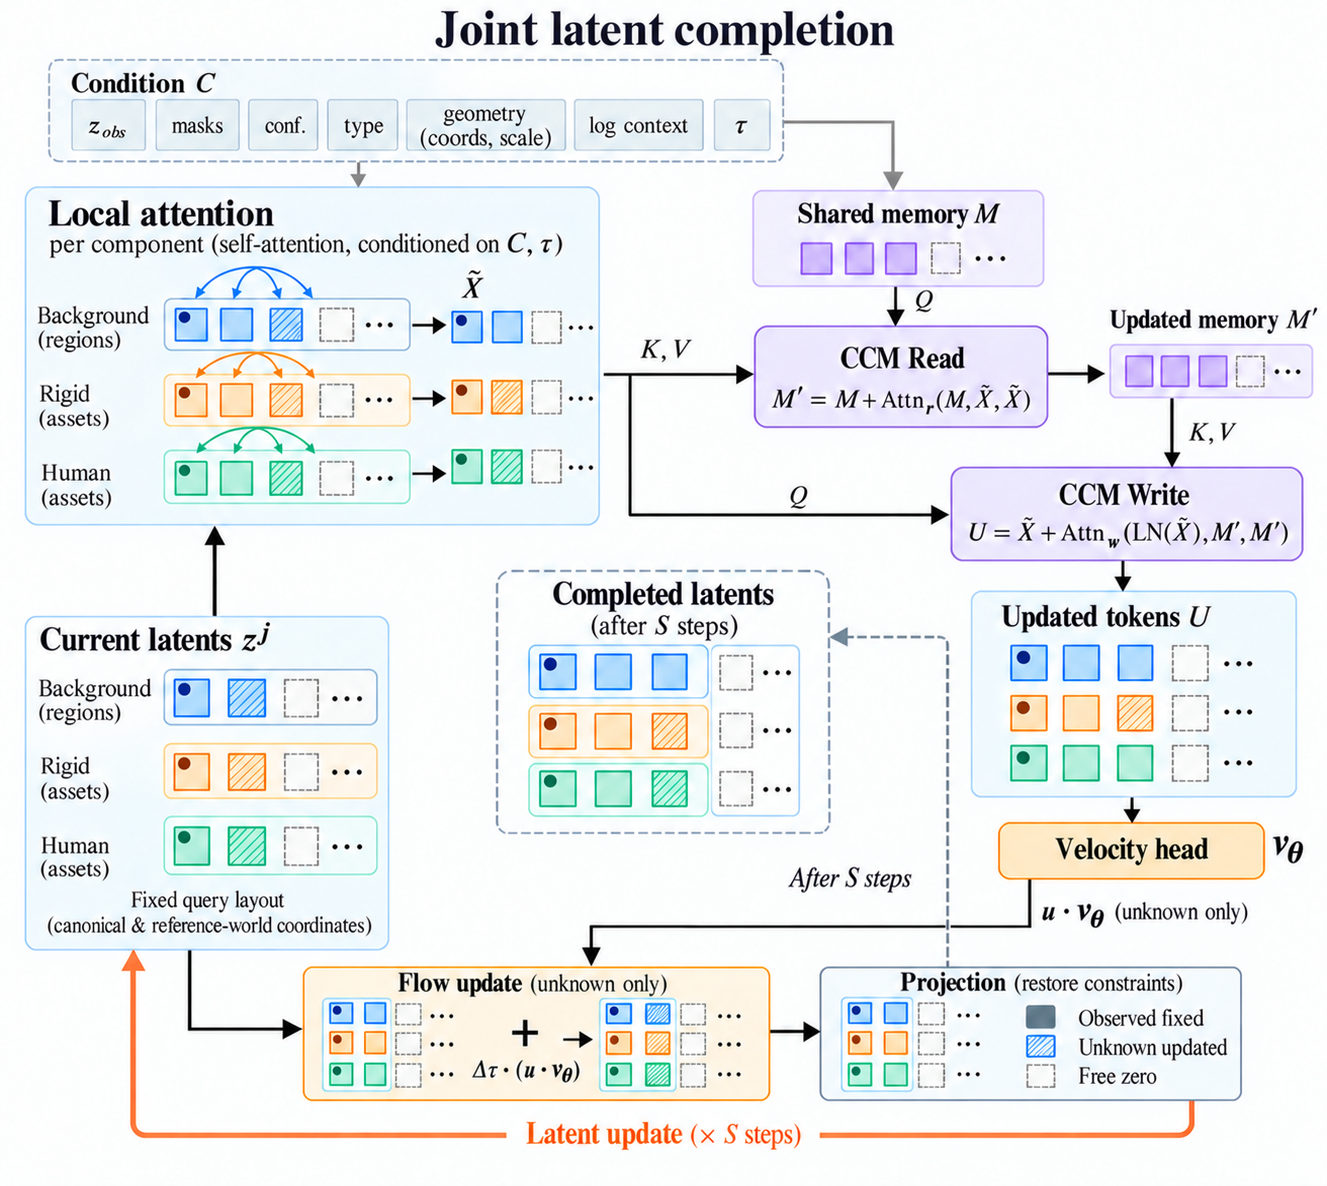
\includegraphics[width=0.86\textwidth]{fig/drivecompose-joint-completion.png}
  \caption{\textbf{Joint latent completion.} Group-local attention updates component features; CCM reads them into shared memory and writes context back to every component. The velocity head drives unknown-code updates. Projection restores observed codes and clears free-space codes after each step, with the query layout fixed. Completed codes are taken after the final projection.}
  \label{fig:joint-completion}
\end{figure*}

\paragraph{Generative completion module.}

Our generative completion module (GCM) combines a scene-conditioned flow transformer with constrained sampling (Fig.~\ref{fig:joint-completion}). We parameterize its completion velocity with a DiT-style transformer~\cite{peebles2023dit} trained by flow matching~\cite{lipman2022flowmatching}. Its input combines current and observed codes, masks, confidence, type, both coordinate descriptions, cell scales, and pooled log features. Background groups follow spatial neighborhoods, each asset forms a local group, and sky directions are grouped by cubemap face. Local self-attention processes these groups separately. A cross-component memory (CCM) module then exchanges context through shared memory:

\begin{align}
\mathbf M'&=\mathbf M+\operatorname{Attn}_{r}
(\mathbf M,\widetilde{\mathbf X},\widetilde{\mathbf X}),\\
\mathbf U&=\widetilde{\mathbf X}+\operatorname{Attn}_{w}
(\operatorname{LN}(\widetilde{\mathbf X}),\mathbf M',\mathbf M').
\label{eq:memory-exchange}
\end{align}

Here $\widetilde{\mathbf X}$ concatenates locally updated tokens, and attention arguments are queries, keys, and values. A residual feed-forward update follows $\mathbf U$. Flow-time modulation enters the local normalization; learned tokens and log summaries initialize memory. This structure keeps each support's local organization while allowing a rigid or human query to use information from the surrounding scene.

\paragraph{Flow training and constrained sampling.}

Let $\mathbf z_1$ be a complete target on the same query layout and $\boldsymbol\epsilon\sim\mathcal N(0,\mathbf I)$ be Gaussian noise. We interpolate only the unknown content at flow time $\tau\in[0,1]$:

\begin{equation}
\mathbf z_\tau=m\odot\mathbf z^{\rm obs}
+u\odot[(1-\tau)\boldsymbol\epsilon+\tau\mathbf z_1].
\label{eq:flow-path}
\end{equation}

Observed codes remain fixed and free-space codes remain zero. The target velocity for unknown queries is $\mathbf z_1-\boldsymbol\epsilon$. With an optional loss selector $s_i$, the objective is

\begin{equation}
\mathcal L_{\rm flow}=
\frac{\sum_i u_i s_i\|\mathbf v_\theta(\mathbf z_\tau,\tau,C)_i
-(\mathbf z_{1,i}-\boldsymbol\epsilon_i)\|_2^2}
{D\max(1,\sum_i u_i s_i)}.
\label{eq:flow-loss}
\end{equation}

Complete scene or asset examples supply $\mathbf z_1$ at the unknown queries, while $s_i$ selects their contribution to the training loss (Sec.~\ref{sec:training}).

At inference, we initialize unknown codes with noise and take $S$ Euler steps with $\Delta\tau=1/S$:

\begin{equation}
\mathbf z^{j+1}=\Pi_{m,f}\!\left[
\mathbf z^j+\Delta\tau\,u\odot
\mathbf v_\theta(\mathbf z^j,j/S,C)\right].
\label{eq:sampling}
\end{equation}

The projection $\Pi_{m,f}$ restores observed codes and clears free-space codes after every step. The seed fixes one sampled completion. Sampling precedes decoding, and the resulting scene is reused when the camera or actor states change.

\subsection{Type-specific Gaussian decoding}
\label{sec:decoding}

Background, rigid, and human Gaussian decoders independently map each query to $K$ child Gaussians confined to its support cell. Human children inherit the query's skinning weights; rigid children share their asset's rigid transform. Opacity is multiplied by $1-f_i$, so free queries cannot produce visible Gaussians. A separate sky head predicts cubemap colors within the observation-supported domain $V_{\rm sky}$. Gaussian and appearance parameterizations are detailed in Appendix E of the supplementary material.

Each query is decoded independently. Freezing the codec and retaining observed codes therefore preserves the Gaussian parameters of observed surfaces.

\subsection{Scene composition}
\label{sec:composition}

\paragraph{State-driven rendering.}

At time step $k$, state $s_k$ specifies the ego pose, active assets, rigid transforms, and human root and joint poses. Rigid poses transform canonical Gaussian centers and covariances rigidly. Human joint poses deform them through the stored skinning weights, so completed surfaces move with the corresponding body parts. Appendix C gives the transformations. The renderer composites the background, active assets, and valid sky:

\begin{equation}
o_k=\mathcal R(\operatorname{Compose}(\mathcal W,s_k),\mathcal C_k).
\label{eq:simulation}
\end{equation}

Changing the camera selects a new view of the composed scene; changing an actor state moves its completed canonical asset. The background and canonical content remain fixed across these operations, allowing the same reconstruction to be reused along different trajectories.

\subsection{Training procedure}
\label{sec:training}

We train visual recovery, the latent codec, and the completion model in sequence, then adapt completion through rendered observations (Table~\ref{tab:training}). Freezing the codec during completion training keeps its target latent space fixed.

\begin{table}[t]
\centering
\small
\caption{Training schedule. R: recovery; C: codec; G: GCM. T: trained; F: frozen; --: unused.}
\label{tab:training}
\begin{tabular}{@{}lccc p{0.43\linewidth}@{}}
\toprule
Stage & R & C & G & Supervision \\
\midrule
Recovery & T & -- & -- & Geometry, semantics, identity, states \\
Codec & F & T & -- & Partial / complete observations \\
Prior & F & F & T & Complete targets \\
Adaptation & F & F & T & Real-log rendering and scene constraints \\
\bottomrule
\end{tabular}
\end{table}

For codec fitting, partial input and more complete observations share the same query positions, types, order, and ownership. With recovery and the entire codec frozen, complete scene or asset examples provide a valid target for every unknown query to train the GCM with Eq.~\ref{eq:flow-loss}. Real-log adaptation differentiates through flow integration, decoding, and rendering to update only the GCM. Complete-target samples can be interleaved to retain the prior, with each loss applied only to samples carrying its required targets. Observed anchors are enforced by frozen decoding and hard code restoration. Detailed supervision, losses, and conditioning perturbations are provided in Appendix B of the supplementary material.

% Frozen verbatim from the supplied MOSAIC archive, by user instruction.
\section{Experiments}
\label{sec:experiments}
We evaluate our method along four axes:
\textit{(i)} dynamic scene reconstruction quality on Waymo Open Dataset,
covering temporal interpolation and extrapolation
(\S~\ref{sec:temporal_evaluation});
\textit{(ii)} off-trajectory view synthesis under lateral
camera shifts (\S~\ref{sec:spatial_evaluation});
\textit{(iii)} cross-dataset transfer from Waymo to nuScenes
(\S~\ref{sec:generalization}); and
\textit{(iv)} ablations of the main design choices
(\S~\ref{sec:ablations}).

\subsection{Experimental Setup}
\label{sec:experimental_setup}

\paragraph{Datasets and protocol.}
We use the Waymo Open Dataset with 798 training and 202 validation sequences. Following STORM, each validation sequence is divided into non-overlapping 2-second clips of 20 frames at 10 \, Hz~\cite{yang2025storm}. The FRONT, FRONT\_LEFT, and FRONT\_RIGHT cameras provide observations at zero-based frame indices $\{0,5,10,15\}$. The remaining 16 frames are used for evaluation: 12 frames for temporal interpolation and four frames for prediction beyond the last observation. Predictions and reference images are resized to $240\times160$ pixels for evaluation~\cite{huang2026instantnurec}.

\paragraph{Baselines.}
We compare with STORM, DGGT, StreetForward~\cite{yang2025storm,chen2025dggt,yu2026streetforward}. Methods use the same context timestamps and target views, with model-specific preprocessing. Camera parameters, additional geometric inputs, and rendering adapters are documented with the implementation settings. For spatial extrapolation, we compare Gaussian renderings before diffusion refinement, following PointForward~\cite{chi2026pointforward}.

\paragraph{Metrics.}
We report PSNR and SSIM over the full image and shared annotated regions. Depth quality is measured using AbsRel and $\delta_1$ at valid projected LiDAR samples after per-frame scale alignment~\cite{huang2026instantnurec}. Scores are averaged over frames within each clip and then over clips within each sequence; sequences receive equal weight. Novel-trajectory renderings are evaluated using FID and FVD against a fixed real-image and video reference population.

\paragraph{Implementation details.}
DriveCompose reconstructs category-specific actor assets from motion-aligned observations and composes them with a static background. Reconstruction time includes preprocessing, asset generation, and scene composition. Rendering time is measured separately, and asset reuse is evaluated across repeated scene queries.
% Fill in verified DriveCompose training schedule, resolution, hardware and checkpoint.
% Do not copy baseline training configurations into DriveCompose implementation details.

\subsection{Dynamic Reconstruction and Temporal Prediction}
\label{sec:temporal_evaluation}

We evaluate reconstruction at unobserved times along the recorded camera trajectory. Table~\ref{tab:regions_current} reports image and depth quality. The regional comparison focuses on actor appearance, and synchronized visualizations examine object position, shape, and occlusion changes.
% Add measured DriveCompose findings here after replacing the development numbers.
\begin{table}[!htbp]
\centering
\footnotesize
\setlength{\tabcolsep}{1.3pt}
\renewcommand{\arraystretch}{1.08}
\setlength{\belowcaptionskip}{5pt}
\caption{Dynamic scene reconstruction on Waymo. Image quality is reported over the full image and annotated regions; depth is evaluated at valid LiDAR samples.}
\label{tab:regions_current}
\begin{tabular}{@{}lrrrrrr@{}}
\toprule
& \multicolumn{2}{c}{Full image} & \multicolumn{2}{c}{\shortstack{Dynamic Region}} & \multicolumn{2}{c}{Depth} \\
\cmidrule(lr){2-3}\cmidrule(lr){4-5}\cmidrule(lr){6-7}
Method & PSNR $\uparrow$ & SSIM $\uparrow$ & PSNR $\uparrow$ & SSIM $\uparrow$ & AbsRel $\downarrow$ & $\delta_1$ $\uparrow$ \\
\midrule
STORM & 26.191 & 0.833 & 22.083 & 0.654 & 0.129 & 0.867 \\
DGGT & 26.056 & 0.809 & 20.809 & 0.603 & 0.168 & 0.779 \\
StreetForward & 25.256 & 0.814 & 21.844 & 0.636 & 0.122 & 0.860 \\
\midrule
DriveCompose & -- & -- & -- & -- & -- & -- \\
\bottomrule
\end{tabular}
\end{table}

\paragraph{Temporal interpolation and prediction.}
Table~\ref{tab:temporal_current} separates temporal interpolation from prediction at 0.1--0.4 seconds beyond the last context frame.

\begin{table}[!htbp]
\centering
\footnotesize
\setlength{\tabcolsep}{1.3pt}
\renewcommand{\arraystretch}{1.08}
\setlength{\belowcaptionskip}{5pt}
\caption{Temporal interpolation and extrapolation on Waymo. PSNR and SSIM are reported separately for interpolation and extrapolation; context frames are excluded.}
\label{tab:temporal_current}
\begin{tabular}{@{}lrrrrrr@{}}
\toprule
& \multicolumn{2}{c}{Interp.} & \multicolumn{2}{c}{Extrap.} & \multicolumn{2}{c}{All targets} \\
\cmidrule(lr){2-3}\cmidrule(lr){4-5}\cmidrule(lr){6-7}
Method & PSNR $\uparrow$ & SSIM $\uparrow$ & PSNR $\uparrow$ & SSIM $\uparrow$ & PSNR $\uparrow$ & SSIM $\uparrow$ \\
\midrule
STORM & 26.427 & 0.842 & 25.481 & 0.807 & 26.191 & 0.833 \\
DGGT & 26.265 & 0.817 & 25.429 & 0.788 & 26.056 & 0.809 \\
StreetForward & 25.653 & 0.827 & 24.065 & 0.776 & 25.256 & 0.814 \\
\midrule
DriveCompose & -- & -- & -- & -- & -- & -- \\
\bottomrule
\end{tabular}
\end{table}

\subsection{Off-Trajectory View Synthesis}
\label{sec:spatial_evaluation}

We shift the camera trajectory laterally by 1, 2, and 4 meters to the left and right, keeping camera orientation, intrinsics, and timestamps fixed. This evaluation tests the stability of scene structure and the rendering of newly visible surfaces as the viewpoint moves away from the observations~\cite{zhu2025worldsplat,chi2026pointforward}.

Table~\ref{tab:spatial_current} reports FID and FVD
at each displacement magnitude, averaged over separately
evaluated left and right shifts. Both metrics use the
same real reference population across methods.
Qualitative comparisons use matched scenes, timestamps,
and camera offsets to examine vehicle shape, road layout,
and occlusion boundaries.

\begin{table}[t]
\centering
\footnotesize
\setlength{\tabcolsep}{2.5pt}
\renewcommand{\arraystretch}{1.08}
\caption{Novel-view synthesis under lateral camera shifts.
FID and FVD are averaged over left and right shifts
at each displacement magnitude. Lower is better.}
\label{tab:spatial_current}
\resizebox{\columnwidth}{!}{%
\begin{tabular}{@{}l|rr|rr|rr@{}}
\toprule
Method
& \multicolumn{2}{c|}{Shift $\pm 1$ m}
& \multicolumn{2}{c|}{Shift $\pm 2$ m}
& \multicolumn{2}{c}{Shift $\pm 4$ m} \\
\cmidrule(lr){2-3}
\cmidrule(lr){4-5}
\cmidrule(lr){6-7}
& FID $\downarrow$ & FVD $\downarrow$
& FID $\downarrow$ & FVD $\downarrow$
& FID $\downarrow$ & FVD $\downarrow$ \\
\midrule
STORM
& 61.97 & 722.27
& 83.72 & 1029.36
& 132.57 & 1704.16 \\
DGGT
& 73.99 & 984.00
& 93.36 & 1197.03
& 128.01 & 1661.70 \\
StreetForward
& 84.30 & 878.95
& 103.31 & 1095.02
& 123.58 & 1578.63 \\
\midrule
\rowcolor{gray!10}
DriveCompose
& -- & --
& -- & --
& -- & -- \\
\bottomrule
\end{tabular}%
}
\end{table}

% Avoid stretching paragraph gaps beside the taller single-column table.
\raggedbottom
\subsection{Cross-Dataset Generalization}
\label{sec:generalization}

We evaluate transfer from Waymo to nuScenes under zero-shot and fine-tuning settings. Zero-shot evaluation directly applies the Waymo-trained checkpoint without target-domain updates. Fine-tuning adapts the same initialization using the nuScenes training split and evaluates it on the held-out validation split. Both settings use the same target evaluation scenes, context sampling, and metrics.

Table~\ref{tab:generalization} reports the two settings separately. The zero-shot comparison assesses transfer to new environments, while the fine-tuning comparison measures adaptation to the target domain. Full-image and annotated-region scores distinguish overall scene quality from actor reconstruction.
% Planned protocol: all cells below are unmeasured. Fill the target split,
% fine-tuning data budget, update count and camera mapping before evaluation.
% Span both columns so the generalization comparison is not stranded in the
% right column beside an empty float area.

\begin{table}[t]
\centering
\footnotesize
\setlength{\tabcolsep}{3.5pt}
\renewcommand{\arraystretch}{1.08}
\caption{Cross-dataset generalization and target-domain adaptation.
Zero-shot models are evaluated directly on the target datasets, while
trained models are fine-tuned on the target domain. Higher PSNR and SSIM,
and lower LPIPS are better.}
\label{tab:generalization}
\begin{tabular*}{\columnwidth}{
    @{\extracolsep{\fill}}l
    ccc@{\hskip 5pt}|@{\hskip 5pt}ccc
}
\toprule
& \multicolumn{3}{c}{\textbf{Full image}}
& \multicolumn{3}{c}{\textbf{Dynamic regions}} \\
\cmidrule(lr){2-4}\cmidrule(lr){5-7}
\textbf{Method}
& PSNR $\uparrow$ & SSIM $\uparrow$ & LPIPS $\downarrow$
& PSNR $\uparrow$ & SSIM $\uparrow$ & LPIPS $\downarrow$ \\
\midrule

\multicolumn{7}{l}{\textbf{Zero-shot}} \\
STORM
& -- & -- & --
& -- & -- & -- \\
DGGT
& -- & -- & --
& -- & -- & -- \\
StreetForward
& -- & -- & --
& -- & -- & -- \\
\rowcolor{gray!12}
\textbf{DriveCompose}
& \textbf{--} & \textbf{--} & \textbf{--}
& \textbf{--} & \textbf{--} & \textbf{--} \\

\midrule
\multicolumn{7}{l}{\textbf{Trained}} \\
STORM
& -- & -- & --
& -- & -- & -- \\
\rowcolor{gray!12}
\textbf{DriveCompose}
& \textbf{--} & \textbf{--} & \textbf{--}
& \textbf{--} & \textbf{--} & \textbf{--} \\

\bottomrule
\end{tabular*}
\end{table}

\subsection{Ablation protocol}
\label{sec:ablation-protocol}
\label{sec:ablations}

\paragraph{Inputs and controls.}
Paired evaluation of hidden surfaces is defined on independent complete-reference scenes; Waymo logs provide recorded-view evaluation.
Each 29-timestamp window uses three synchronized cameras: front, front-left, and front-right.
The nested input sets are $\mathcal T_2=\{0,28\}$, $\mathcal T_4=\{0,8,20,28\}$, and $\mathcal T_8=\{0,4,\ldots,28\}$, with shared target timestamps $\{2,6,\ldots,26\}$.
Target images are excluded from evidence and query construction; target camera and actor states are supplied equally to every variant.
The recovery module and codec are frozen, with matched query layouts, data exposure, and optimization budgets at each input setting.
Training samples $T\in\{2,4,8\}$ uniformly; completion uses 24 Euler steps.
The four learned variants use training seeds $\{0,1,2\}$ and world seeds $\{7,17,27\}$; A1 is deterministic.
Hyperparameters and acceptance thresholds are selected on an internal development split before evaluation on scene- and identity-disjoint data.

\paragraph{Metrics.}
New-MAE measures linear-RGB error on independently identified surfaces unseen in every input; NVS-MAE covers all held-out target pixels.
Across input settings, New-MAE uses the common region unseen even under $\mathcal T_8$.
Obs-Reg averages the positive input-view regression in Eq.~\ref{eq:regression}.
Cov.\ is the non-sky target fraction with support coverage $>0.5$, opacity $>0.1$, and finite positive depth.
Uncovered pixels receive the same zero-RGB fill for error measurement.
Pass is the fraction of all requested worlds accepted by the fixed checker, including construction failures in its denominator.
Image metrics include every renderable candidate, including rejected worlds; non-renderable counts are recorded separately.
Metrics are averaged within each scene and then across scenes and training seeds.

Figure~\ref{fig:ablation-reuse} reserves matched crops for completion and observation preservation, followed by three state interventions from the same world.

\begin{figure*}[t]
  \centering
  \begingroup
  \newcommand{\dcablationcell}[3]{%
    \begin{minipage}[t]{#1}
      \centering
      \parbox[c][2.2\baselineskip][c]{\linewidth}{\centering\small #3}\par
      \fbox{\rule{0pt}{#2}\rule{.90\linewidth}{0pt}}
    \end{minipage}}
  {\small\textbf{(a) Unseen-surface completion}}\par\smallskip
  \dcablationcell{.158\textwidth}{12mm}{GT}\hfill
  \dcablationcell{.158\textwidth}{12mm}{No completion\\(A1)}\hfill
  \dcablationcell{.158\textwidth}{12mm}{Independent\\(A2)}\hfill
  \dcablationcell{.158\textwidth}{12mm}{No world coord.\\(A3)}\hfill
  \dcablationcell{.158\textwidth}{12mm}{Soft observation\\(A7)}\hfill
  \dcablationcell{.158\textwidth}{12mm}{Full\\(A0)}
  \par\medskip
  {\small\textbf{(b) Input-view preservation}}\par\smallskip
  \dcablationcell{.158\textwidth}{12mm}{GT / Input}\hfill
  \dcablationcell{.158\textwidth}{12mm}{No completion\\(A1)}\hfill
  \dcablationcell{.158\textwidth}{12mm}{Independent\\(A2)}\hfill
  \dcablationcell{.158\textwidth}{12mm}{No world coord.\\(A3)}\hfill
  \dcablationcell{.158\textwidth}{12mm}{Soft observation\\(A7)}\hfill
  \dcablationcell{.158\textwidth}{12mm}{Full\\(A0)}
  \par\medskip
  {\small\textbf{(c) One fixed world, different states (A0)}}\par\smallskip
  \dcablationcell{.235\textwidth}{20mm}{Original $s_0$}\hfill
  \dcablationcell{.235\textwidth}{20mm}{Camera $+1\,\mathrm m$}\hfill
  \dcablationcell{.235\textwidth}{20mm}{Vehicle $+30^\circ$}\hfill
  \dcablationcell{.235\textwidth}{20mm}{Human pose $H_1$}
  \endgroup
  \caption{\textbf{Ablation and reuse layout.} (a) The same newly exposed region across five variants and an independent reference. (b) Matched crops in an original input view. (c) Independent camera, vehicle, and human-state changes from one A0 world with seed 7; the other states and lighting are fixed. All image slots are intentionally empty.}
  \label{fig:ablation-reuse}
\end{figure*}

\subsection{Ablation studies}
\label{sec:ablation-studies}

\paragraph{Completion and scene context.}
Table~\ref{tab:ablation-components} compares Full (A0) with three controls.
No completion (A1) disables the opacity of every non-observed, non-sky query.
Independent (A2) isolates component memories at every layer while sharing parameters and retaining the same global log context.
No world coord.\ (A3) zeros only the explicit reference-world coordinate channels in the completion network; canonical geometry and rendering transforms remain unchanged.
The learned controls are retrained through Stages 3--4; memory-related compute differences are recorded.

\paragraph{Observation preservation.}
Soft observation (A7) allows observed codes to evolve instead of hard resetting them.
Its observed flow path is $(1-\tau)\mathbf z^{\rm obs}+\tau\mathbf z_1$, with target velocity $\mathbf z_1-\mathbf z^{\rm obs}$.
Observed and unknown flow losses are separately normalized and equally weighted.
Rendering adaptation adds a mean-squared penalty on observed-code changes, with its weight selected from $\{0.1,1,10\}$ on development data.
Observed conditioning, free-space constraints, the codec, and the checker remain fixed.
This comparison examines the tradeoff between completion and input-view preservation.

\begin{table}[t]
  \centering
  \caption{\textbf{Component ablations.} All variants use $T=8$, a shared recovery module and codec, and the same evaluation masks. Quality is measured before acceptance filtering; Pass includes all requested worlds. A1 requires no completion training. Numerical cells are left blank.}
  \label{tab:ablation-components}
  \small
  \setlength{\tabcolsep}{3pt}
  \begin{tabular}{@{}lrrrr@{}}
    \toprule
    Variant & \shortstack{New-MAE\\$\downarrow$}
      & \shortstack{Obs-Reg\\$\downarrow$}
      & \shortstack{Cov.\\(\%) $\uparrow$}
      & \shortstack{Pass\\(\%) $\uparrow$}\\
    \midrule
    Full (A0)            & & & & \\
    No completion (A1)   & & & & \\
    Independent (A2)     & & & & \\
    No world coord. (A3) & & & & \\
    Soft obs. (A7)       & & & & \\
    \bottomrule
  \end{tabular}
\end{table}

\paragraph{Input sparsity.}
Table~\ref{tab:ablation-inputs} reuses the A0/A2 checkpoints at $T=2,4,8$, with 6/12/24 input images.
The time span, target views, and common unseen-region mask remain fixed; evidence and queries are rebuilt from each input subset.
No model is retrained for this comparison.

\begin{table}[t]
  \centering
  \caption{\textbf{Input-timestamp sensitivity.} Three cameras and a fixed time span are shared across the nested input sets. The same checkpoints and target images are used at every $T$; New-MAE uses the common unseen region. Numerical cells are left blank.}
  \label{tab:ablation-inputs}
  \small
  \setlength{\tabcolsep}{3pt}
  \begin{tabular}{@{}lr rrr@{}}
    \toprule
    Variant & $T$ & \shortstack{NVS-MAE\\$\downarrow$}
      & \shortstack{New-MAE\\$\downarrow$}
      & \shortstack{Cov.\\(\%) $\uparrow$}\\
    \midrule
    Full (A0)        & 2 & & & \\
    Independent (A2) & 2 & & & \\
    Full (A0)        & 4 & & & \\
    Independent (A2) & 4 & & & \\
    Full (A0)        & 8 & & & \\
    Independent (A2) & 8 & & & \\
    \bottomrule
  \end{tabular}
\end{table}

\subsection{State-driven reuse}
\label{sec:ablation-reuse}


At timestamp 14 and world seed 7, the interventions independently translate the camera by $1\,\mathrm m$ along its local $+x$ axis, rotate a vehicle by $30^\circ$ about its root and the world vertical axis, or apply a held-out valid human pose $H_1$ with fixed root placement.
Lighting and canonical assets remain fixed, without resampling completion.

% Flush experiment floats before Discussion and Conclusion.
\FloatBarrier

\FloatBarrier
\Needspace{13\baselineskip}
\section{Discussion}
\label{sec:discussion}

DriveCompose separates canonical scene content from camera and actor states. Its representation covers a finite region under fixed illumination, with rigid vehicles and humans bound to a fixed skeleton and clothing volume. Depth, identity, and canonical-pose estimates determine the observed anchors used by completion, so recovery errors propagate into the reconstructed geometry. Human articulation follows the template's geometric support, and contact and collision behavior are handled by the physical simulator. Relighting and changes in clothing geometry require corresponding appearance and deformation models.

\Needspace{17\baselineskip}
\section{Conclusion}
\label{sec:conclusion}

DriveCompose jointly completes world-space background and canonical actor latents, preserving component identity and motion bindings for state-driven reuse. Shared scene context improves missing-surface reconstruction, while fixed Gaussian assets support camera shifts, vehicle rotation, and human pose edits. Waymo reconstruction, paired hidden-surface tests, and real-scene edits demonstrate the quality and reuse of the completed content.
\label{sec:main-text-end}

\FloatBarrier
{\small
\bibliographystyle{ieeenat_fullname}
\bibliography{main}
}
\end{document}
